\section{Test cases}

\paragraph{}
In iteration 3, we will attempt to get to be able to run the individual requests:

\begin{itemize}
    \item Clone, update, push a repository with authentication
    \item Get a response to the git-lfs-authenticate command
    \item Get a response to the /objects/batch api call
\end{itemize}

\paragraph{}
Testing will be done from a client container, that will access other containers in the network. The result of this container will be the result of the tests.

\subsection{The test runner}

\paragraph{}
The scenario we will discuss here rely on architecture. Most of it is to test connections between a client and some servers, or between servers themselves. To achieve that, deploying an actual infrastructure would be too much work. Instead, this project rely on the docker abstractions to simulate the networks.

\paragraph{}
The test runner is a container that will run the tests. It has a volume pointing to the tests folder (a set of shell files). It is included in architectures defined by docker compose files, so it can access the other containers.

\paragraph{}
To run the test \textit{014\_test\_case\_abc.sh}, the idea is to run

\begin{lstlisting}[language=bash]
    docker-compose 
        -f architectures/default.docker-compose.yaml 
        run tester_client 
        bash /root/run_test.sh 14
\end{lstlisting}

\paragraph{}
The tester\_client container will run the test, format the output and print it to the console.

\paragraph{}
To make it easier and format this output in the flow of docker related output, the script \textit{start.sh} is available and is the recommended way to run the tests. It also handle cleanup and formatting of the output. It requires bash to run\footnote{We use PIPESTATUS to be able to get the output of the docker run command streaming to a formatting function and retrieve the exit code}.



\subsection{Test case 1: Clone, update, push a repository with authentication}
\subsubsection{Description}
\begin{wrapfigure}{r}{0.5\textwidth}
    \begin{center}
        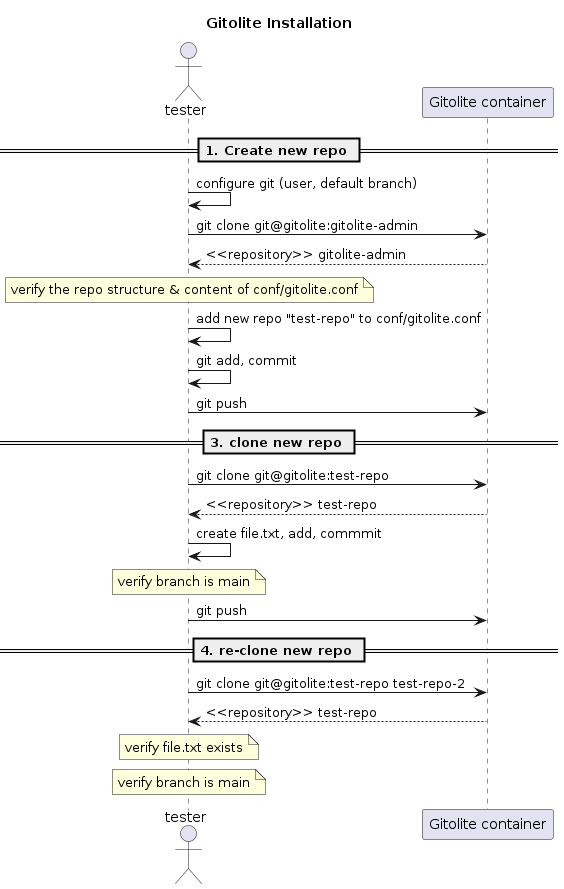
\includegraphics[width=0.45\textwidth]{prototyping/diagrams/gitolite_installation_verification}
    \end{center}
    \caption{Test case 1}
\end{wrapfigure}


\paragraph{}
As an admin, I shall be able to clone the admin repo, add a new repo, add, commit and push my changes.

\paragraph{}
Then, I shall be able to clone the new repo, add a file, add, commit and push my changes. As I configured by default branch to main, my first commit shall be on main.

\paragraph{}
Then, if I clone a second time the repo, I shall be able to see the file I added.

\subsubsection{Architecture}

\paragraph{}
The architecture has two containers:

\begin{itemize}
    \item A client container, that will run the tests
    \item A gitolite server container, that will run the server
\end{itemize}

\subsubsection{Implementation}

\paragraph{}
Implementation of test and images revealed that with non-standard default branch (for instance "main"), the second clone of the repository is not working well. It is cloned, but an invalid refspec is warned. Inspired by \url{https://gist.github.com/schnell18/8f31feb03e211c6fa4f1}, we added a set-head post create hook to gitolite.

\paragraph{}
Artifacts for the authentication module are:

\begin{itemize}
    \item \textit{/modules/auth/Dockerfile}, the image containing gitolite, with \textit{docker-entrypoint.sh} and \textit{set-head} scripts
    \item \textit{/tests/tests/01\_gitolite\_clone.sh}, the test script, using the \textit{/tests/architectures/default.docker-compose.yaml} architecture
\end{itemize}

\subsection{Test case 2: Get a response to the git-lfs-authenticate command}

\subsubsection{Description}
\begin{wrapfigure}{r}{0.6\textwidth}
    \begin{center}
        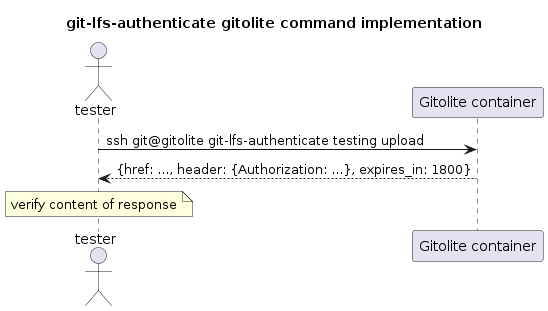
\includegraphics[width=0.55\textwidth]{prototyping/diagrams/gitolite_lfs_authenticate}
    \end{center}
    \caption{Test case 2}
\end{wrapfigure}


The first step of the git-lfs protocol is to authenticate. The client sends a request to the server, and the server responds with a token and an href. The client then uses this token to authenticate to the server. This behavior takes place in the gitolite server, not the lfs server, as it is the gitolite server that knows the users and is then able to sign the tokens. 

Let's test that even without the lfs server, so we are sure that the authentication module is working.

\subsubsection{Architecture}

\paragraph{}
We can keep the same architecture, with just the gitolite server and the tester

\subsubsection{Implementation}

\paragraph{}
Expected artifacts are:

\begin{itemize}
    \item the updated image (Dockerfile, entrypoint, ...)
    \item the git-lfs-authenticate command implementation
    \item \textit{/tests/tests/02\_git\_lfs\_authenticate.sh}, the test script, using the default architecture
\end{itemize}

\newpage
\subsection{Test case 3: Get a response to the /objects/batch api call}

\subsubsection{Description}

\begin{wrapfigure}{r}{0.5\textwidth}
    \begin{center}
        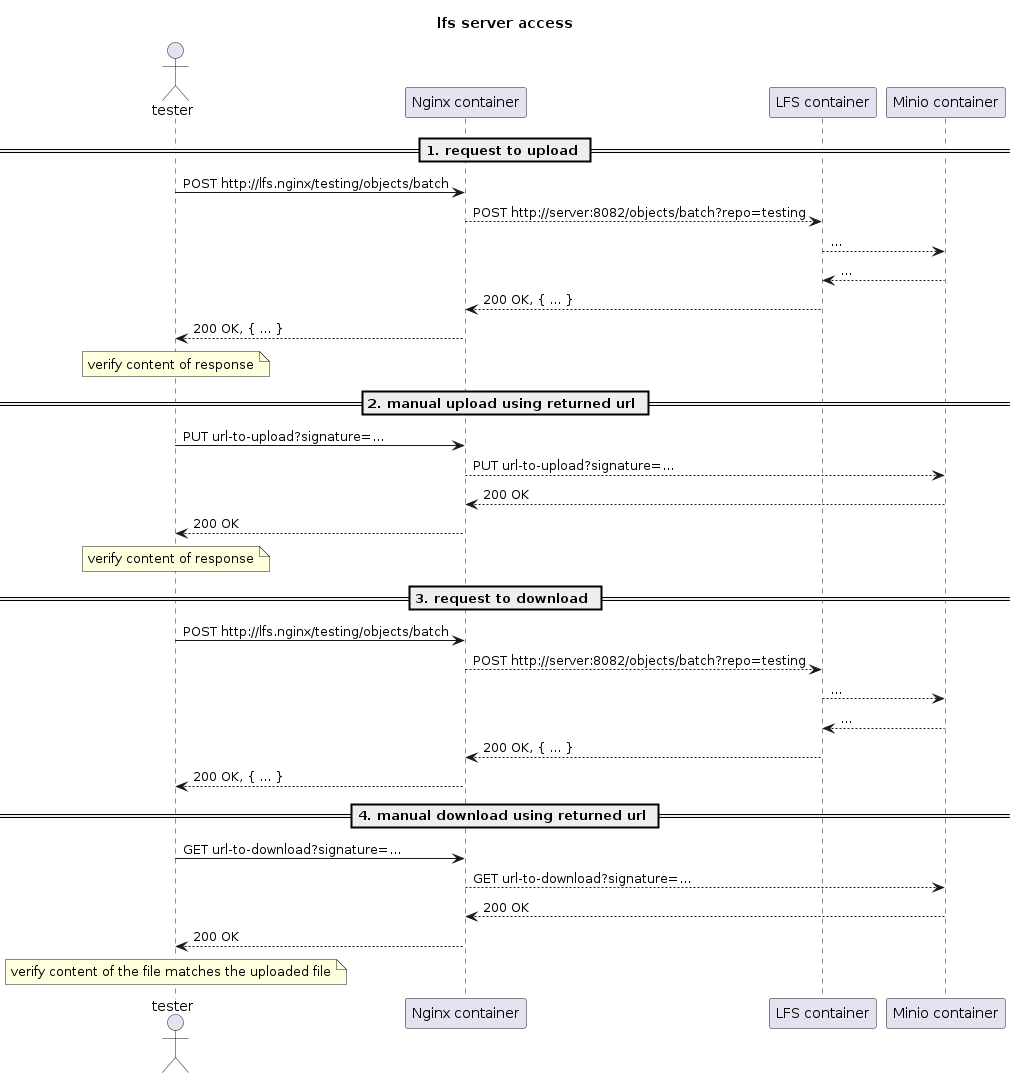
\includegraphics[width=0.45\textwidth]{prototyping/diagrams/lfs_server_access}
    \end{center}
    \caption{Test case 3}
\end{wrapfigure}

Then, we will develop a first implementation of the /objects/batch api call. This call is used by the client to get the list of objects to upload or download. The client sends a request to the server, and the server responds with a list of metadata informing the client of how to download/upload the given files. It also provides signed links to the client, so that the client can download/upload the files.

The test case will assume that the links are generated by the lfs server, but the files are actually stored in minio, and the links are directly handled by minio. 

\subsubsection{Architecture}
We will add a few more containers

\begin{itemize}
    \item A minio server, that will store the files
    \item A lfs server, that will generate the links
    \item An nginx server, that will expose the minio server and the lfs server
\end{itemize}

\subsubsection{Implementation}

\paragraph{}
Expected artifacts are:

\begin{itemize}
    \item a basic server implementing the /objects/batch api  (jwt verification, metadata generation, link generation), assuming links are handled by minio
    \item the image for the lfs server
    \item the new architecture file
    \item \textit{/tests/tests/03\_lfs\_batch.sh}, the test script
\end{itemize}
